\documentclass[a4paper]{article}

\usepackage{authblk}
\usepackage[utf8x]{inputenc}
\usepackage[T1]{fontenc}
\usepackage{textcomp}
\usepackage[romanian]{babel}
\usepackage{indentfirst}
\usepackage{amssymb}
\usepackage{amsmath}
\usepackage{amsthm}
\usepackage{mathtools}
\usepackage{listings}
\usepackage{lmodern}
\usepackage[romanian]{babel}
\usepackage{amsmath}
\usepackage{listings}
\usepackage{graphicx}
\usepackage{cite}


\theoremstyle{remark}
\newtheorem{remark}{Observa\c{t}ia}
\newtheorem{theorem}{Teorema}[section]
\newtheorem{lemma}[theorem]{Lema}
\newtheorem{proposition}[theorem]{Propozi\c{t}ia}
\newtheorem{corollary}[theorem]{Corolarul}
\theoremstyle{definition}
\newtheorem{definition}{Defini\c{t}ia}[section]
\newtheorem{example}{Exemplul}[section]

\def\o1{$\mathcal{O}(1)$}

\title{\textbf{Cuckoo Hashing}}
\author{Vlad-Doru Ion}
\date{16 Decembrie 2014}
\affil{Facultatea de Matematica si Informatica \\ Universitatea din Bucuresti}

\begin{document}

\maketitle

\section{Introducere}

Cuckoo Hashing este numele unui un algoritm de hashing ce a fost descris de Rasmus Pagh și Flemming Friche Rodler în Ianuarie 2002. Numele acestui provine de la pasărea \textit{Cuckoo} care împinge celalte ouă afară din cuib după ce a spart oul său. Acest proces reprezintă o analogie pentru algoritmul de inserare pe care îl vom prezenta.

Algoritmul descrie construcția unei tabele de dispersie ce permite regăsirea informației în complexitate timp \o1. În ceea ce privește complexitatea spațiu a algoritmului aceasta este apropiată de ce a arborilor binari de căutare.

Spre deosebire de algoritmul de hashing dinamic perfect, propus de Dietzfelbinger, a cărui performanță o egalează în ceea ce privește complexitatea timp, Cuckoo hashing propune o implementare elegantă și care se dovedește a fi foarte utilă în practică.

\subsection {Obiective}

Vom enumera obiectivele pe care le urmărește algoritmul pentru a le putea observa în construcția algoritmului.
\begin{itemize}
\item Complexitatea timp a operației de căutare: $\mathcal{O}(1)$
\item Complexitatea timp a operației de inserare: $\mathcal{O}(1)$ amorizat\footnote{Complexitatea amoritzată ia în considerare cazul cel mai rău pe o secvență de operații, asigurându-se astfel că cele cu o complexitate ridicată au o frecvență scazută.}
\item Spațiu utilizat de tabelel de disperise: $\approx 2n$
\end{itemize}

\subsection {Ideea centrală}

Majoritatea algoritmilor folosesc o singură funcție de hashing, apoi tratează in diferite moduri coliziunile.

\textit{Cuckoo hashing} alege o abordare diferită față de cea clasică, și va folosi două funcții de hashing. În plus el va pune constrângerea ca fiecare cheie să se afle la doar una din cele două locații indicate de funcțiile alese, obținând căutare în timp constant. 

\begin{remark}
Datorită faptului că cele două funcții de hashing sunt independente, accesul la memorie poate fi făcut în mod paralel pe procesoarele care suportă acest lucru, îmbunătățind performanță a algoritmului în practică.
\end{remark}

\section {Preliminarii}

În cele ce urmează vom prezenta o serie de elemente fundamentele pentru a construi discuția în jurul algoritmului \textit{Cuckoo Hashing}.

Pe parcursul acestui lucrări, când ne vom referi la chei, ne vom referi la elementele unei mulțimi $U = {0,1}^w$, unde $w$ reprezintă dimensiunea cuvântului asociat procesorului. În general cheile vor fi elemente întregi reprezentate pe 32 de biți.

Dacă unei chei nu îi corespunde nicio valoare atunci vom nota acest lucru prin simbolul $\bot$.

Algoritmul va folosi cele două funcții de hash alese dintr-o \textit{familie universală} de funcții de hashing.

\begin{definition}
O familie  $h_i, i \in I, h_i:D \to E$  este \textit{$(c,k)$-universală} dacă, $\forall k > 0, \forall x_1, x_2 ..., x_k \in U \text{ distincte}, \forall y_1, ..., y_k \in E,$ și $i$ ales uniform peste $I$ atunci: \\ \[Pr[h_i(x1) = y1, ..., h_i(x_k) = y_k] \leq \frac{c}{|E|^k}\]
\end{definition}

\section {Descrierea algortimului}

După cum am precizat anterior algoritmul va folosi două funcții de hashing pe care le vom nota cu $h1$, respectiv $h2$. Pentru a stoca cheile vom folosi două tabele $T1$ și $T2$, acestea având aceeași dimensiune pe care o vom nota cu $r$. Astfel funcția $h1$ va atribui unei chei $x$ poziția $h1(x)$ din tabela $T1$, în timp ce funcția $h2$ va atribui, în mod analog, poziția $h2(x)$ din tabela $T2$. Avem astfel definiția formală:

\[h_1, h_2: U \to \{0, 1, ..., r-1\}\]

\begin{remark}
Oricare cheie $x$ se va găsi fie în celula $h1(x)$ a tabelei $T1$, fie în celula $h2(x)$ a tabelei $T2$, \textbf{dar niciodată în ambele}.
\end{remark}

\subsection{Căutarea și ștergerea unei chei}

Având în vedere modul de stocare a cheilor descris anterior putem deduce în mod trivial funcția de căutare.\footnote{Vom descrie funcția folosind limbajul de programare \textit{Python} întrucât acesta este unul intuitiv.}

\begin{verbatim}
  def lookup(x):
   	return T1[h1(x)] == x or T2[h2[x]] == x
\end{verbatim}

Este evident că avem o complexitate timp $\mathcal{O}(1)$ deoarece efectuăm două operații de acces la memorie ce se produc în timp constant.

Pentru ștergerea unei chei putem presupune fară pierderea generalității ca avem o cheie $x$ ce se află în tabelul $T1$. Atunci vom șterge cheia x prim marcarea poziției $h_1(x)$ din T1 ca fiind nefolosita: $T1[h_1(x)] := \bot$. Funcția de ștergere urmează același raționament.

\begin{verbatim}
  def erase(x):
    if T1[h1(x)] == x:
   	  T1[h1(x)] = None
   	if T2[h2[x]] == x:
   	  T2[h2(x) = None
\end{verbatim}

\subsection{Inserarea unei chei}

Vom presupune ca va trebui sa inserăm cheia $x$. Deoarece ea nu poate fi pusă decât la una din pozițiile menționate anterior trebuie găsită o strategie de inserare în concordanță cu această constrângere.

\begin{itemize}
  \item[Cazul 1] Dacă $T1[h_1(x)] == \bot$ atunci inserăm cheia $x$ la poziția $h1(x)$. STOP.
  \item[Cazul 2] Dacă $T1[h_1(x)] == y$ atunci inserăm cheia $x$ la poziția $h1(x)$. Iterăm prin a insera cheia $y$ în tabelul T2 folosind același raționament.
\end{itemize}

\begin{remark}Există posibilitatea de a intra într-un ciclu folosind mecanismul de inserare. De aceea numărul de iterații va fi mărginit de o constantă superioară. În momentul în care constanta este atinsă vom alege două noi funcții de hashing și vom reinsera toate cheile.
\end{remark}

În figura de mai jos putem vedea o ilustrare grafică a modului în care se inserează o cheie $x$. În partea stangă se poate observa structura înainte de inserare, iar în partea dreaptă după.

\begin{figure}[h]
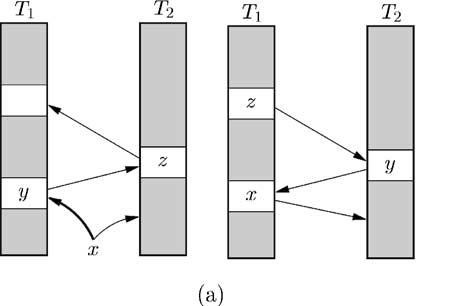
\includegraphics[width=0.4\linewidth]{cuckoo.jpg}
\end{figure}

Săgețile din fiecare cheie reprezintă pozițiile corespunzătoare acestora în tabelele T1 și T2. 

\newpage

\subsection{Implementarea funcției de inserare}

Vom prezenta în cele ce urmează codul corespunzător acestei funcții de inserare.

\begin{verbatim}
  def insert(x):
  	# Verificam daca cheia exista deja.
  	if lookup(x):
  		return
   	for i in range(MaxLoop):
   	  T1[h1[x]], x = x, T1[h1[x]]
   	  if x == None:
   	    return
   	  T2[h2[x]], x = x, T2[h2[x]]
   	  if x == None:
   	    return
   	# Daca nu am putut face inserarea
   	rehash()
   	insert(x)
\end{verbatim}

\section{Variante de implementare}

Se pot elabora diferite variante de implementare a algoritmului prezentat plecând de la diferite observații. O primă variantă are la bază observația că algoritmul incearcă întâi să insereze în tabela T1. Din acest motiv putem folosi tabele de dimensiuni \textbf{asimetrice}, crescând dimensiunea tabelei T1.

O altă variantă este aceea de a folosi o singură tabela T de dimensiune $2r$ pentru ambele functii de hashing.

\begin{remark}
Pentru eleganță ultimei variante putem considera ca poziții fezabile pentru $x$ locațiile $h_1(x), (h_2(x) - h_1(x)) \mod 2r$. În acest mod putem sări de la o locație la alta folosind funcția $i \to (h_2(x) - i) \mod 2r$. Acest lucru se poate verifica ușor înlocuind pe i cu fiecare din locațiile posibile pentru $x$.
\end{remark}

\subsection{Analiza complexității}

Deoarece am concluzionat că operățiile de inserare și ștergere au o complexitate timp de $\mathcal{O}(1)$ vom analiza în cele ce urmează comportamentul operației de inserare care nu este unul trivial.

\begin{lemma}
\footnote{Demonstrația este una complexă și nu face subiectul acestei prezentări.}
Presupunem că procedura de inserare nu intră într-un ciclu infinit. Atunci pentru orice prefix $x_1, x_2, ..., x_p$ al secvenței de chei mutate de către procedură, există o secvența de \textbf{cel puțin $\frac{p}{3}$} chei consecutive fară repetiții, începând cu cheia $x_1$.
\end{lemma}.

Lucrarea originală în care este prezentat algoritmul demonstreaza că probabilitatea de a cauza apelarea procedurii de rehash este de $\mathcal{O}(1/n^2)$. În particular fiecare operație de inserție ce este efectuată în cadrul procedurii de rehashing are o probabilitate de succes de $1 - \mathcal{O}(1/n)$. Obținem astfel un timp mediu pentru procedura de rehashing de complexitate $\mathcal{O}(n)$ 

În cele din urmă combinând rezultatele expuse reiese că pentru fiecare inserție timpul mediu pentru rehashing este de $\mathcal{O}(1/n)$, considerând șî apelare forțată a procedurii de rehashing o dată la $r^2$ inserări.

În concluzie am arătat că acest algoritm prezintă o complexitate $\mathcal{O}(1)$ amortizat pentru operație de inserare a unei chei.

\section {Concluzii}

În final vom prezenta conluziile obținute bazate pe descrierea și analiza complexității algoritmului de hashing \textit{Cuckoo Hashing}.

\begin{itemize}

\item Am prezentat un algoritm cu complexitate constantă la căutarea unei chei, pe cazul cel mai defavorabil.

\item Algoritmul este unul elegant și simplu de implementat și prezintă mai multe variante ale acestuia.

\item Algoritmul se comportă excelent în practică.

\end{itemize}

\newpage

\nocite{*}

\bibliography{referat.bib}{}
\bibliographystyle{plain}

\end{document}
